\begin{frame}
    \frametitle{Giới thiệu ma trận}
    \[ \mathbf{A}=
\begin{bmatrix}
    1&5&12\\
    3&0&4\\
    0&7&9
\end{bmatrix}
\]
\[\mathbf{B}=\begin{bmatrix}
    -1.3&0.6\\
    20.4&5.5\\
    9.7&-6.2
\end{bmatrix}\]
Quy tắc đọc: hàng trước cột sau.\newline
\(\mathbf{A}_{21}=3\).\newline
\(\mathbf{B}_{32}=-6.2\).
\end{frame}
\begin{frame}
    \frametitle{Ma trận 1 cột}
    Ví dụ:
    \[\mathbf{v}=\begin{bmatrix}
    a\\b\\c
\end{bmatrix}, \quad \mathbf{w}=\begin{bmatrix}
    c\\d\\f
\end{bmatrix}.\]
\end{frame}
\begin{frame}
    \frametitle{Ma trận 1 cột}
    Ví dụ: 
    \[\mathbf{v}=\begin{bmatrix}
    a\\b\\c
\end{bmatrix}, \quad \mathbf{w}=\begin{bmatrix}
    c\\d\\f
\end{bmatrix}.\]
Nếu,
\[\mathbf{v}+\mathbf{w}=\begin{bmatrix}
    a+c\\b+d\\c+f
\end{bmatrix},\qquad
    n\cdot\mathbf{v}=\begin{bmatrix}
        na\\nb\\nc
\end{bmatrix}.\] \[\implies \text{Vector}\]
\end{frame}
\begin{frame}
    \frametitle{Chuyển đổi ký hiệu}
    \[(a,b,c)\rightarrow \begin{bmatrix}
    a\\b\\c
\end{bmatrix}\]
\begin{figure}[H]
    \centering
    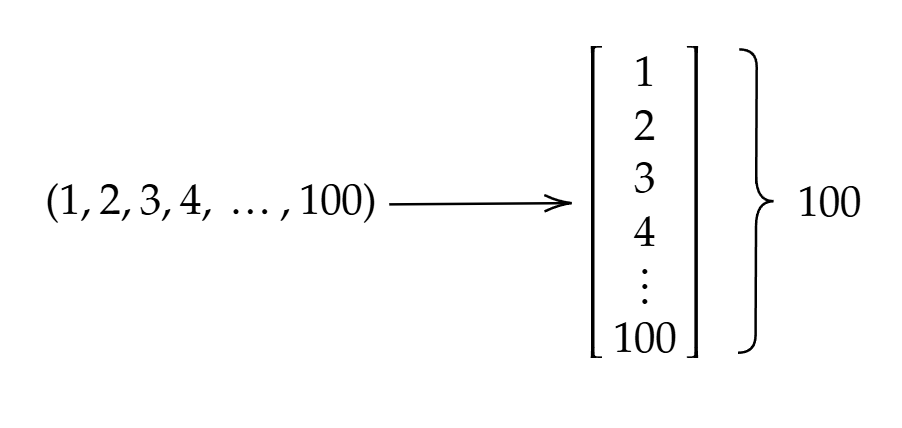
\includegraphics[width=9cm, height=4cm]{Slides/Figure/array100.png}
\end{figure}
\end{frame}
\begin{frame}
    \frametitle{Dạng tổng quát của một ma trận}
    Một ma trận m hàng n cột về tổng quát có dạng:
    \[\mathbf{A}_{m\times n}=\begin{bmatrix}
    \mathbf{A}_{11} &   \mathbf{A}_{12} &\cdots &\mathbf{A}_{1j} &\cdots      & \mathbf{A}_{1n}\\  
    \mathbf{A}_{21} &   \mathbf{A}_{22} &\cdots &\mathbf{A}_{2j} &\cdots      & \mathbf{A}_{2n}\\
    \vdots          &   \vdots          &\ddots &\vdots          &\ddots      & \vdots         \\
    \mathbf{A}_{i1} &   \mathbf{A}_{i2} &\cdots &\mathbf{A}_{ij} &\cdots      & \mathbf{A}_{in}\\
    \vdots          &   \vdots          &\ddots &\vdots          &\ddots      &\vdots          \\
    \mathbf{A}_{m1} &   \mathbf{A}_{m2} &\cdots &\mathbf{A}_{mj} &\cdots      & \mathbf{A}_{mn}              
\end{bmatrix}.\]
\end{frame}
\begin{frame}
    \frametitle{Các phép toán trên ma trận}
    \textbf{Phép cộng ma trận.} \[(\mathbf{A}+\mathbf{B})_{ij}=\mathbf{A}_{ij}+\mathbf{B}_{ij}.\]
    \textbf{Phép nhân ma trận với một số.}\[(c\mathbf{A})_{ij}=c\mathbf{A}_{ij}.\]
    Ví dụ: \[4\begin{bmatrix}
    0&3\\ 2&-6
\end{bmatrix}+\begin{bmatrix}
    1&-2\\ 0&5
\end{bmatrix}=??\]
\end{frame}
\begin{frame}
    \frametitle{Các phép toán trên ma trận}
    \textbf{Phép cộng ma trận.} \[(\mathbf{A}+\mathbf{B})_{ij}=\mathbf{A}_{ij}+\mathbf{B}_{ij}.\]
    \textbf{Phép nhân ma trận với một số.}\[(c\mathbf{A})_{ij}=c\mathbf{A}_{ij}.\]
    Ví dụ: \[4\begin{bmatrix}
    0&3\\ 2&-6
\end{bmatrix}+\begin{bmatrix}
    1&-2\\ 0&5
\end{bmatrix}=\begin{bmatrix}
    0&12\\ 8&-24
\end{bmatrix}+\begin{bmatrix}
    1&-2\\ 0&5
\end{bmatrix}=\begin{bmatrix}
    1&10\\ 8&-19
\end{bmatrix}.\]
\end{frame}
\begin{frame}
    \frametitle{Các phép toán trên ma trận}
    Cho \[\mathbf{v}=\begin{bmatrix}
    +2\\+5\\-4
\end{bmatrix}.\] Phân tích trong một hệ cơ sở ngẫu nhiên,
\[\begin{bmatrix}
    2\\5\\-4
\end{bmatrix}=\alpha\begin{bmatrix}
    1\\0\\0
\end{bmatrix}+\beta\begin{bmatrix}
    0\\2\\-5
\end{bmatrix}+\gamma\begin{bmatrix}
    0\\11\\-19
\end{bmatrix}.\]
\end{frame}
\begin{frame}
    \frametitle{Các phép toán trên ma trận}
    Cho \[\mathbf{v}=\begin{bmatrix}
    +2\\+5\\-4
\end{bmatrix}.\] Phân tích trong một hệ cơ sở ngẫu nhiên,
\[\begin{bmatrix}
    2\\5\\-4
\end{bmatrix}=\alpha\begin{bmatrix}
    1\\0\\0
\end{bmatrix}+\beta\begin{bmatrix}
    0\\2\\-5
\end{bmatrix}+\gamma\begin{bmatrix}
    0\\11\\-19
\end{bmatrix}.\]
Tính được \((\alpha,\beta,\gamma)=(2,-3,1)\).
\end{frame}
\begin{frame}
    \frametitle{Các phép toán trên ma trận}
    \textbf{Phép nhân ma trận-vector.}
    \[\begin{bmatrix}
    2\\5\\-4
\end{bmatrix}=2\begin{bmatrix}
    1\\0\\0
\end{bmatrix}+(-3)\begin{bmatrix}
    0\\2\\-5
\end{bmatrix}+1\begin{bmatrix}
    0\\11\\-19
\end{bmatrix}.\]
    \[\begin{bmatrix}
    2\\5\\-4
\end{bmatrix}=\begin{bmatrix}
    1&0&0\\
    0&2&11\\
    0&-5&-19
\end{bmatrix}\begin{bmatrix}
    2\\-3\\1
\end{bmatrix}.\]
\end{frame}
\begin{frame}
    \frametitle{Các phép toán trên ma trận}
    \textbf{Phép nhân ma trận-vector.}\begin{equation}\label{eq1}
    \begin{bmatrix}
    2\\5\\-4
\end{bmatrix}=\begin{bmatrix}
    1&0&0\\
    0&2&11\\
    0&-5&-19
\end{bmatrix}\begin{bmatrix}
    2\\-3\\1
\end{bmatrix}.\end{equation}
Một ma trận \(m\times n\) nhân với một vector n thành phần = một vector m thành phần; phần tử thú i của vector:
\begin{equation}
    (\mathbf{Ax})_i = \sum_{j=1}^n \mathbf{A}_{ij}\mathbf{x}_j.
\end{equation}
\end{frame}
\begin{frame}
    \frametitle{Phép nhân ma trận-vector}
    Phần tử thứ \(i\) của vector này là tích vô hướng của hàng thứ \(i\) của \(\mathbf{A}\) với vector \(\mathbf{x}\). Chẳng hạn,
    \[\begin{bmatrix}
    0&2&11
\end{bmatrix}\begin{bmatrix}
    2\\-3\\1
\end{bmatrix}=\begin{bmatrix}
    0\\2\\11
\end{bmatrix}\cdot \begin{bmatrix}
    2\\-3\\1
\end{bmatrix}=0\times 2+2\times(-3)+11\times 1 =5.\]
\end{frame}
\begin{frame}
    \frametitle{Phép nhân ma trận-vector}
    Tóm gọn:\[\begin{bmatrix}
    \vert &\vert&\vert\\
    \mathbf{A}_{i1}&\mathbf{A}_{i2}&\mathbf{A}_{i3}\\
    \vert &\vert&\vert\\
\end{bmatrix}\begin{bmatrix}
    x_1\\x_2\\x_3
\end{bmatrix}=x_1\begin{bmatrix}
    \vert\\\mathbf{A}_{i1}\\ \vert
\end{bmatrix}+x_2 \begin{bmatrix}
    \vert\\\mathbf{A}_{i2}\\ \vert
\end{bmatrix}+x_3\begin{bmatrix}
    \vert\\\mathbf{A}_{i1}\\ \vert
\end{bmatrix}.\]
Tính phân phối: \[\mathbf{A}(\mathbf{a}+\mathbf{b})=\mathbf{A}\mathbf{a}+\mathbf{A}\mathbf{b}.\]
\end{frame}
\begin{frame}
    \frametitle{Phép nhân ma trận với ma trận}
    \[
    \begin{bmatrix}
    1\\0\\0
    \end{bmatrix}=1\begin{bmatrix}
    0.5 \\-1\\0
    \end{bmatrix}+2\begin{bmatrix}
    0.75 \\1\\-2
    \end{bmatrix}+1\begin{bmatrix}
    -1 \\-1\\4
    \end{bmatrix}\]\[\rightarrow \begin{bmatrix}
        1\\0\\0
    \end{bmatrix}=\begin{bmatrix}
        0.5 & 0.75 & -1\\
        -1 & 1 & -1\\
        0 & -2 & 4
    \end{bmatrix}\begin{bmatrix} 1\\2\\1\end{bmatrix}.
    \]
\end{frame}
\begin{frame}
    \frametitle{Phép nhân ma trận với ma trận}
    \[
    \begin{bmatrix}
    0\\2\\-5
\end{bmatrix}=-1.625\begin{bmatrix}
    0.5\\-1\\0
\end{bmatrix}-1.75\begin{bmatrix}
    0.75\\-1\\0
\end{bmatrix}-2.125\begin{bmatrix}
    -1\\-1\\4
\end{bmatrix}\]\[\rightarrow \begin{bmatrix}
    0\\2\\-5
\end{bmatrix}=\begin{bmatrix}
    0.5 & 0.75 & -1\\
    -1 & 1 & -1\\
    0 & -2 & 4
\end{bmatrix}\begin{bmatrix}
    -1.625\\-1.75\\-2.125
\end{bmatrix}.
\]
\end{frame}
\begin{frame}
    \frametitle{Phép nhân ma trận với ma trận}
    \[
    \begin{bmatrix}
    0\\11\\-19
\end{bmatrix}=-7.875\begin{bmatrix}
    0.5\\-1\\0
\end{bmatrix}-3.25\begin{bmatrix}
    0.75\\-1\\0
\end{bmatrix}-6.375\begin{bmatrix}
    -1\\-1\\4
\end{bmatrix}
    \]
    \[\rightarrow
    \begin{bmatrix}
    0\\11\\-19
\end{bmatrix}=\begin{bmatrix}
    0.5 & 0.75 & -1\\
    -1 & 1 & -1\\
    0 & -2 & 4
\end{bmatrix}\begin{bmatrix}
    -7.875\\-3.25\\-6.375
\end{bmatrix}.
    \]
\end{frame}
\begin{frame}
    \frametitle{Phép nhân ma trận với ma trận}
    Đặt
    \[\begin{bmatrix}
    0.5 & 0.75 & -1\\
    -1 & 1 & -1\\
    0 & -2 & 4
\end{bmatrix}=\mathbf{B}.\] Thay 3 đẳng thức trên vào \ref{eq1},
\[\begin{bmatrix}
    2\\5\\-4
\end{bmatrix}=\begin{bmatrix}
    \mathbf{B}\begin{bmatrix}
        1\\2\\1
    \end{bmatrix}&\mathbf{B}\begin{bmatrix}
        -1.625\\-1.75\\-2.125
    \end{bmatrix}&\mathbf{B}\begin{bmatrix}
        -7.875\\-3.25\\-6.375
\end{bmatrix}\end{bmatrix}\begin{bmatrix}
2\\-3\\1
\end{bmatrix}.\]
Sự lặp lại của \(\mathbf{B}\)(!)
\end{frame}
\begin{frame}
    \frametitle{Phép nhân ma trận với ma trận}
    Tạo ra một phép toán mới để:
    \begin{equation}\label{eqmatrix}\begin{bmatrix}
    2\\5\\-4
\end{bmatrix}=\mathbf{B}\begin{bmatrix}
    1&-1.625&-7.875\\
    2&-1.75&-3.25\\
    1&-2.125&-6.375
\end{bmatrix}\begin{bmatrix}
    2\\-3\\1
\end{bmatrix}\end{equation}
\begin{tcolorbox}[colback=blue!10!, colframe=blue!50!black]
    Xét một ma trận \(\mathbf{A}_{m\times n}\) và một ma trận \(\mathbf{B}_{n\times p}\), \emph{tích của của chúng là một ma trận \(\mathbf{C}_{m\times p}\); các cột của ma trận này là các vector, bằng với tích ma trận-vector của ma trận \(\mathbf{A}\) và các cột tương ứng  của ma trận \(B\).}
\end{tcolorbox}
    Tương đương điều này, \begin{equation}\label{eq4}
    \mathbf{C}_{ij}=(\mathbf{AB})_{ij}=\sum_{k=1}^n \mathbf{A}_{ik}\mathbf{B}_{kj}.\end{equation}
\end{frame}
\begin{frame}
    \frametitle{Phép nhân ma trận với ma trận}
\begin{figure}[H]
    \centering
    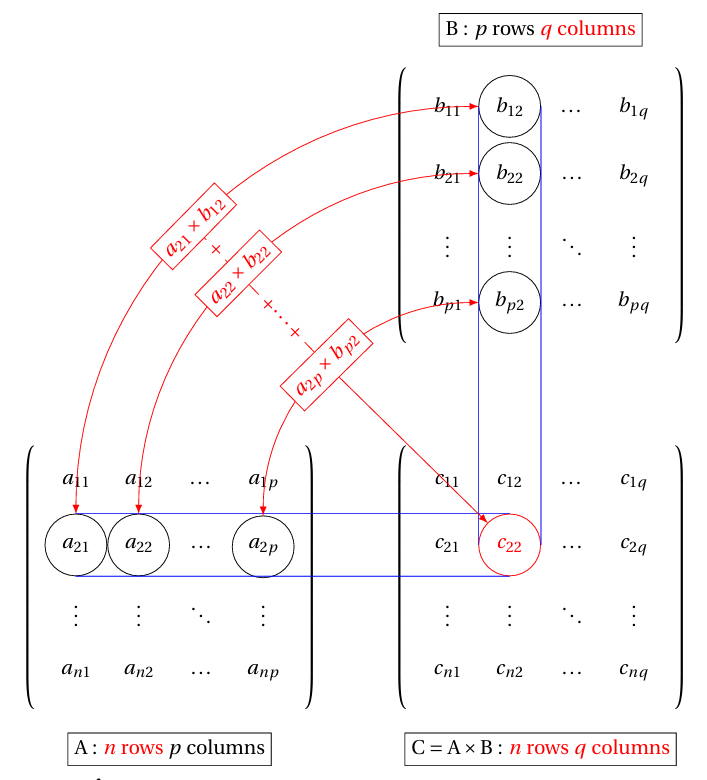
\includegraphics[width=6cm, height=6cm]{Slides/Figure/matricemultiplication.png}
\end{figure}
\end{frame}
\begin{frame}
    \frametitle{Ví dụ}
    Tính tích \[\begin{bmatrix}
    1&5\\ 3&2
\end{bmatrix}\begin{bmatrix}
    2&-1\\ 0&3
\end{bmatrix}\] theo hai cách: \eqref{eq4} và bằng góc nhìn của phép nhân vector.
\end{frame}
\begin{frame}
    \frametitle{Ví dụ- Giải}
    Cách 1: \[\begin{bmatrix}
    (1\cdot 2+5\cdot 0)&(1\cdot -1+5\cdot 3)\\
   ( 3\cdot 2+2\cdot 0)&(3\cdot -1+2\cdot 3)
\end{bmatrix}=\begin{bmatrix}
    2&14\\
    6&3
\end{bmatrix}.\]
\end{frame}
\begin{frame}
    \frametitle{Ví dụ-Giải}
    Cách 2: Theo góc nhìn của phép nhân vector, tích này tương đương với 
\[\begin{bmatrix}
    \begin{bmatrix}
        1&5\\3&2
    \end{bmatrix}\begin{bmatrix}
        2\\0
    \end{bmatrix} &\begin{bmatrix}
        1&5\\3&2
    \end{bmatrix}\begin{bmatrix}
        -1\\3
    \end{bmatrix}
\end{bmatrix}.\]
Dễ thấy, \begin{align*}
    &\begin{bmatrix}
        1&5\\3&2
    \end{bmatrix}\begin{bmatrix}
        2\\0
    \end{bmatrix}=2\begin{bmatrix}
        1\\3
    \end{bmatrix}+0\begin{bmatrix}
        5\\2
    \end{bmatrix}=\begin{bmatrix}
        2\\6
    \end{bmatrix},\\
    &\begin{bmatrix}
        1&5\\3&2
    \end{bmatrix}\begin{bmatrix}
        -1\\3
    \end{bmatrix}=-1\begin{bmatrix}
        1\\3
    \end{bmatrix}+3\begin{bmatrix}
        5\\2
    \end{bmatrix}=\begin{bmatrix}
        14\\3
    \end{bmatrix}.
\end{align*}
\end{frame}
\begin{frame}
    \frametitle{Các phép toán trên ma trận}
    \textbf{Các quy tắc cho các phép toán trên ma trận.} Ta tổng kết lại các quy tắc chung nhất.
    \begin{enumerate}
    \item Quy luật giao hoán: \(\mathbf{A}+\mathbf{B}=\mathbf{B}+\mathbf{A}\).
    \item Quy luật phân phối: \(\alpha(\mathbf{A}+\mathbf{B})=\alpha\mathbf{A}+\alpha\mathbf{B}\).
    \item Quy luật liên kết: \(\mathbf{A}+(\mathbf{B}+\mathbf{C})=(\mathbf{A}+\mathbf{B})+\mathbf{C}\).
    \item Quy luật liên kết: \((\mathbf{AB})\mathbf{C}=\mathbf{A}(\mathbf{BC})\).
    \item Quy luật phân phối (trái): \(\mathbf{A}(\mathbf{B}+\mathbf{C})=\mathbf{AB}+\mathbf{AC}\).
    \item Quy luật phân phối (phải): \((\mathbf{A}+\mathbf{B})\mathbf{C}=\mathbf{AC}+\mathbf{BC}\).
    \item Quy luật giao hoán: \(\mathbf{AB} \neq \mathbf{BA}\).
\end{enumerate}
Chú ý quy luật cuối cùng, tích ma trận không mang tính giao hoán.
\end{frame}
\begin{frame}
    \frametitle{Phép chuyển vị}
    \begin{tcolorbox}[colback=blue!10, colframe=blue!50!black]
        Ma trận chuyển vị của ma trận \(\mathbf{A}\), ký hiệu là \(\mathbf{A}^T\), là ma trận có các thành phần sao cho \[(\mathbf{A}^T)_{ij}=\mathbf{A}_{ji}.\]
    \end{tcolorbox}
    \[\mathbf{A}=\begin{bmatrix}
    1&2\\3&4
\end{bmatrix}\implies \mathbf{A}^T =\begin{bmatrix}
    1&3\\2&4
\end{bmatrix}.\]
\end{frame}
\begin{frame}
    \frametitle{Tính chất của ma trận chuyển vị}
    \begin{enumerate}
        \item Chuyển vị của phép nhân ma trận
        \[(\mathbf{AB})^T =\mathbf{B}^T \mathbf{A}^T .\]
        \item Tích vô hướng của hai vector được biểu diễn trong hệ cơ sở trực chuẩn
        \[\mathbf{v}\cdot \mathbf{u}=\mathbf{v}^T \mathbf{u}=\mathbf{u}^T \mathbf{v}.\] 
    \end{enumerate}
    \emph{Ví dụ.}
    \[\begin{bmatrix}
    1\\2
\end{bmatrix}\cdot\begin{bmatrix}
    -1\\3
\end{bmatrix}=\begin{bmatrix}
    1&2
\end{bmatrix}\begin{bmatrix}
    -1\\3
\end{bmatrix}=5.\]
\end{frame}